\documentclass[titlepage, a4paper]{article}
\usepackage{hyperref}
\usepackage{graphicx}
\usepackage[utf8]{inputenc}
\usepackage[english]{babel}


\title{
	Quarto! Minimax player \\
	IT3105 \\
}
\author{
	Nordmoen, Jørgen H. \\
	Østensen, Trond
}

\date{\today}

\begin{document}
\pagenumbering{RomanType}
\maketitle

\begin{abstract}\label{abstract}
	This paper is an introduction to our Quarto! minimax player. In this we will try to
	explain how we created our implementation, what sort of decisions the player makes
	the reasoning behind it and our result both against other configurations of our player
	and against other students minimax implementations.
\end{abstract}

\newpage
\tableofcontents

\pagenumbering{arabic}

\section{Introduction}\label{intro}
The game of Quarto!\footnote{Explanation of rules in video form: 
\url{https://www.youtube.com/watch?feature=player_embedded&v=P6dy2eaYmos#!}}
is a quite simple game regarding its rules, but the hard part
comes into play when us humans try to remember all the different attributes of the
game. This is where a game playing algorithm comes into play. With an algorithm
memory no longer becomes an issue as the algorithm can enumerate, if possible, and search
through the whole instance space. In this assignment
we were tasked with creating a minimax\footnote{Explanation of minimax from Wikipedia:
\url{https://en.wikipedia.org/wiki/Minimax}} player with Alpha-beta pruning\footnote{
Further explanation on Wikipedia: \url{https://en.wikipedia.org/wiki/Alpha-beta_pruning}}.
The algorithm it self is not the most difficult one to implement, thats not to say that
we didn't need to debug our code, but the challenge is coming up with a good set of
heuristics to evaluate an intermediate state. We will first introduce our implementation
in a birds eye view, we will then explain our chosen heuristics in more detail before
we move on to our experience in the tournament. Lastly we will describe our results, both
against our own implementation and our tournament results.

\section{Heuristics}\label{heuristics}

\begin{figure}[htb]
	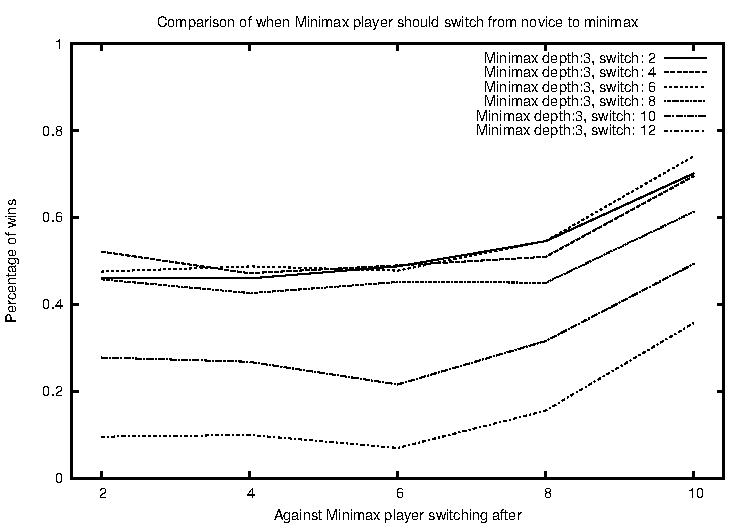
\includegraphics{graphs/switch.pdf}
	\label{fig:minimax switch}
	\caption{Graph describing our minimax switch results}
\end{figure}

\section{Tournament}\label{tournament}

\section{Results}\label{results}

\subsection{Local}\label{results:local}

\subsection{Tournament}\label{results:tournament}

%\section{Future work}\label{future}

\end{document}
